%Clase del documento, tamaño de fuente y hoja
\documentclass[11pt,a4paper]{report}

%paquete para español
\usepackage[utf8]{inputenc}   % input encoding (accents, ñ, etc.)
\usepackage[T1]{fontenc} %output encoding
\usepackage[spanish]{babel}

%paquetes de operadores matematicos
\usepackage{amsmath}
\usepackage{nccmath}

%paquetes para gráficar
\usepackage{graphicx}
\usepackage{subcaption}
\usepackage{tikz}
\usetikzlibrary{arrows.meta,positioning,fit,backgrounds}

%paquete para listar código
\usepackage{listings}
\usepackage{xcolor}
\usepackage{booktabs}
\usepackage{tabularx}
\usepackage{array}

%New colors defined below
\definecolor{codegreen}{rgb}{0,0.6,0}
\definecolor{codegray}{rgb}{0.5,0.5,0.5}
\definecolor{codepurple}{rgb}{0.58,0,0.82}
\definecolor{backcolour}{rgb}{0.95,0.95,0.92}

%Code listing style named "mystyle"
\lstdefinestyle{mystyle}{
  backgroundcolor=\color{backcolour}, commentstyle=\color{codegreen},
  keywordstyle=\color{magenta},
  numberstyle=\tiny\color{codegray},
  stringstyle=\color{codepurple},
  basicstyle=\ttfamily\footnotesize,
  breakatwhitespace=false,
  breaklines=true,
  captionpos=b,
  keepspaces=true,
  numbers=left,
  numbersep=5pt,
  showspaces=false,
  showstringspaces=false,
  showtabs=false,
  tabsize=2
}
%"mystyle" code listing set
\lstset{style=mystyle}

%Para modificacion de titulos
\usepackage{titlesec}

%Ajustar margenes a 2.54cm
\usepackage[margin=1.0in]{geometry}

% diferentes entradas para listas enumeradas
\usepackage{enumitem}
\setlist{itemsep=1pt,topsep=3pt}
% Soporte para buenas urls e hipervínculos entre secciones
\usepackage{hyperref}
\usepackage{bookmark}

%%%%%%%%%%%%%%%%%%%%%%%%%%%%%%%%%%%%%
% Espacio reservado para imágenes que hay que agregar a mano.
% Uso: \placeholder{ancho}{alto}{texto}. Reemplazar por \includegraphics.
\newcommand{\placeholder}[3]{%
  \fbox{\parbox[c][#2][c]{#1}{\centering\small\itshape\color{gray}[IMAGEN PENDIENTE]\\[2pt]#3}}}
%%%%%%%%%%%%%%%%%%%%%%%%%%%%%%%%%%%%%
% Definicion de titulos de la portada
\def \unidad{Universidad de Concepción}
\def \facultad{Facultad de Ingeniería}
\def \departamento{Departamento de Ingeniería Eléctrica}
\def \curso{Taller de Integración TIC}
\def \profe{Luciano Ignacio Radrigán Figueroa}
\def \titulo{Tarea 1}
\def \subtitulo{Sistema de adquisición remota de aceleración\\ESP32-S3 + BMI270 gestionado desde Raspberry Pi}
\def \autores{
    Matthias Aliaga Febres\\
    Joaquin Alonso Lozano Alamo
}
\def \fechalugar{Concepción, \today}
%%%%%%%%%%%%%%%%%%%%%%%%%%%%%%%%%%%%%%

%Quitar "Capitulo X" antes de cada capítulo
\titleformat{\chapter}[display]
  {\normalfont\bfseries}{}{0pt}{\LARGE}
\titlespacing*{\chapter}{0pt}{6pt}{8pt}
% Los capítulos no empiezan en página nueva (informe de máx. 5-6 páginas)
\usepackage{etoolbox}
\makeatletter
\patchcmd{\chapter}{\if@openright\cleardoublepage\else\clearpage\fi}{\par\medskip}{}{}
\makeatother

%%%%%%%%%%%%%%%%%%%%%%%%%%%%%%%%%%%%%%
% Inicia el documento
\setlength{\parindent}{0pt}
\setlength{\parskip}{4pt}

\begin{document}
\pagenumbering{roman}
\renewcommand{\lstlistingname}{Código}
\renewcommand{\tablename}{Tabla}
\renewcommand{\listtablename}{Índice de tablas}
\begin{titlepage}
    \begin{center}
        \vspace*{1cm}

        
\includegraphics[width=0.8\linewidth]{figuras/logos.png}\\
        \vspace{1cm}
        \Huge
        \textbf{\unidad}\\
        \LARGE
        \facultad\\
        \departamento

        \vspace{2cm}

        \LARGE
        \textbf{\curso} \\
        \Large
        \profe\\
        \vspace{2cm}
        \Huge
        \textbf{\titulo}\\
        \vspace{0.1cm}
        \Large
        \autores

        \vfill

        \fechalugar


    \end{center}
\end{titlepage}%


\chapter*{Resumen}
\addcontentsline{toc}{chapter}{Resumen}
Este informe describe el sistema de adquisición remota de aceleración desarrollado para la Tarea 1 del Taller de Integración TIC (TIC3). Un ESP32-S3 lee el acelerómetro BMI270 por I$^2$C y envía las muestras por WiFi a una Raspberry Pi, que actúa como punto de acceso, servidor de sockets y servidor web. Desde una interfaz web en la Raspberry se configuran el rango, la frecuencia de muestreo, el modo de lectura (secuencial o paralelo), el protocolo de transporte (TCP o UDP) y la duración de cada sesión; los datos se grafican en tiempo real y se guardan en la carpeta \texttt{sensores/}.

Se explican la arquitectura, el protocolo binario diseñado y las decisiones que permiten operar a la frecuencia máxima del sensor (1600~Hz): la lectura por la FIFO del BMI270, el aumento del bus I$^2$C a 400~kHz y el envío por lotes (\textit{batching}) en UDP. Con el diseño final se reciben las 1617 muestras/s que entrega realmente el sensor, sin pérdidas en TCP ni en UDP. Finalmente, se comparan ambos protocolos mediante capturas de Wireshark y se analiza el efecto del rango y la frecuencia de muestreo sobre los datos.

\break

\tableofcontents

\clearpage
\setcounter{chapter}{0}
\pagenumbering{arabic}

%=====================================================================
\chapter{Introducción y requisitos}\label{cap:intro}
%=====================================================================
Se desarrolló un sistema de adquisición remota de aceleración: un ESP32-S3 lee el BMI270 por I$^2$C y envía las muestras por WiFi a una Raspberry Pi, que emite la red, aloja el servidor y ofrece una GUI web para configurar, graficar y guardar los datos. La Tabla~\ref{tab:rf} indica cómo se cumple cada requisito funcional.

\begin{table}[h]
\centering\small
\caption{Requisitos funcionales y su implementación.}\label{tab:rf}
\begin{tabularx}{\textwidth}{@{}lX@{}}
\toprule
RF1 & Lectura de los 3 ejes por I$^2$C (400~kHz) desde la FIFO del BMI270. \\
RF2/RF3 & Modo secuencial (una tarea lee y luego envía) y paralelo (tarea lectora en el núcleo 1 + tarea emisora, unidas por una cola FreeRTOS). \\
RF4/RF5 & La Raspberry emite la red (\texttt{10.42.0.0/24}, Pi = \texttt{10.42.0.1}) y es siempre el servidor; el ESP32 siempre inicia las conexiones. \\
RF6/RF7 & Mensaje CONFIG con transporte (TCP por defecto), modo, frecuencia, rango y cantidad de muestras o duración, elegidos en cada sesión. \\
RF8 & GUI web en la Raspberry (puerto 8080): configuración, gráfico en vivo y archivos CSV/JSON en \texttt{sensores/}. \\
RF9 & Capturas de Wireshark de sesiones TCP y UDP a 100 y 1600~Hz (Sección~\ref{sec:wireshark}). \\ \bottomrule
\end{tabularx}
\end{table}

%=====================================================================
\chapter{Arquitectura y protocolo}\label{cap:arquitectura}
%=====================================================================
La Figura~\ref{fig:topologia} muestra la topología: dos enlaces físicos (I$^2$C y WiFi) y tres canales lógicos. El ESP32 inicia las conexiones porque conoce la IP fija de la Raspberry, mientras que su propia IP la asigna el DHCP.

\begin{figure}[h]
\centering
\begin{tikzpicture}[
  blk/.style={draw, rounded corners=3pt, minimum height=0.7cm, align=center, font=\footnotesize, fill=white},
  grp/.style={draw, rounded corners=6pt, inner sep=5pt, fill=gray!8},
  phys/.style={line width=2.2pt, gray!70},
  logic/.style={-{Latex[length=2mm]}, thick, blue!70!black},
  lbl/.style={font=\scriptsize, align=center}]
  \node[blk, fill=blue!6] (bmi) {BMI270\\\scriptsize FIFO 2 KB};
  \node[blk, right=1.3cm of bmi, text width=2.5cm] (fifo) {\texttt{fifo\_take}};
  \node[blk, above=0.2cm of fifo, text width=2.5cm] (cs) {socket control};
  \node[blk, above=0.2cm of cs, text width=2.5cm] (ds) {socket datos};
  \node[blk, below=0.2cm of fifo, text width=2.5cm] (wsta) {WiFi estación};
  \begin{scope}[on background layer]
    \node[grp, fit=(ds)(wsta), label={[font=\footnotesize\bfseries]above:ESP32-S3 (cliente)}] {};
  \end{scope}
  \node[blk, right=2.4cm of ds, text width=2.8cm] (pd) {datos \texttt{:10000}};
  \node[blk, below=0.2cm of pd, text width=2.8cm] (pc) {control \texttt{:10001}};
  \node[blk, below=0.2cm of pc, text width=2.8cm] (st) {\texttt{SampleTracker}, CSV};
  \node[blk, below=0.2cm of st, text width=2.8cm] (ap) {Punto de acceso};
  \node[blk, below=0.2cm of ap, text width=2.8cm] (web) {GUI web \texttt{:8080}};
  \begin{scope}[on background layer]
    \node[grp, fit=(pd)(web), label={[font=\footnotesize\bfseries]above:Raspberry Pi (servidor)}] {};
  \end{scope}
  \node[blk, right=0.9cm of web, fill=blue!6] (nav) {Navegador};
  \draw[phys] (bmi) -- node[lbl, above]{I$^2$C} (fifo);
  \draw[phys] (wsta.east) -- node[lbl, below, pos=0.45]{WiFi WPA2} (ap.west);
  \draw[logic] (ds) -- node[lbl, above]{TCP o UDP} (pd);
  \draw[logic, {Latex[length=2mm]}-{Latex[length=2mm]}] (cs.east) -- node[lbl, above, pos=0.35]{TCP} (pc.west);
  \draw[logic] (web) -- node[lbl, above]{HTTP} (nav);
\end{tikzpicture}
\caption{Topología. En gris, enlaces físicos; en azul, canales lógicos (comparten la misma radio).}
\label{fig:topologia}
\end{figure}

\textbf{Dos canales hacia el ESP32.} Los mensajes de control son pocos y no pueden perderse; las muestras son muchas y su transporte debe ser elegible (RF6). Por eso el control va siempre por TCP, en una conexión que el ESP32 abre al arrancar y mantiene entre sesiones, y el canal de datos se abre en cada sesión con el transporte pedido. Así, elegir UDP nunca arriesga la configuración ni el cierre, y el canal de datos solo transporta muestras, sin byte de tipo.

\textbf{Protocolo binario} (Tabla~\ref{tab:mensajes}). Mensajes de tamaño fijo, little-endian y sin relleno: estructuras \texttt{packed} con \texttt{\_Static\_assert} en C y prefijo \texttt{'<'} de \texttt{struct} en Python (sin él, CONFIG ocuparía 12 bytes en vez de 9). Una muestra ocupa 14 bytes frente a unos 60 en JSON; el ESP32 no formatea texto y la Raspberry decodifica con un solo \texttt{struct.unpack}. El tamaño fijo resuelve el entramado: TCP es un flujo sin límites entre mensajes, por lo que se leen exactamente 14 bytes (\texttt{recv\_exact}); en UDP cada datagrama se corta en trozos de 14. Los ejes se envían crudos (\texttt{int16}, 6 bytes en vez de 12) y la Raspberry los convierte con el rango que configuró:
\begin{equation}
  a\,[\text{m/s}^2] = \text{crudo}\cdot\frac{\text{rango}\cdot 9{,}80665}{32768}.
  \label{eq:escala}
\end{equation}
\texttt{seq} numera cada muestra desde 0 y permite contar muestras perdidas, tardías y duplicadas, también en UDP y también si se pierden antes de la red. El \texttt{total} de END permite calcular la pérdida en el modo por tiempo, y STOP (\texttt{0xFE}) no se confunde con el primer byte de CONFIG (2/4/8/16), así que un STOP tardío se reconoce y descarta.

\begin{table}[h]
\centering\small
\caption{Mensajes del protocolo.}\label{tab:mensajes}
\begin{tabularx}{\textwidth}{@{}l l c X@{}}
\toprule
Mensaje & Canal y sentido & Bytes & Contenido \\ \midrule
CONFIG & control, Pi $\to$ ESP32 & 9 & rango, código de frecuencia (registro), transporte, modo, tipo de fin, límite (\texttt{uint32}) \\
ACK & control, ESP32 $\to$ Pi & 1 & 0 = aceptada; 1--7 = campo inválido \\
DATA & datos, ESP32 $\to$ Pi & 14 & \texttt{seq}, \texttt{t\_us} (\texttt{uint32}); $a_x, a_y, a_z$ crudos (\texttt{int16}) \\
STOP & control, Pi $\to$ ESP32 & 1 & \texttt{0xFE} \\
END & control, ESP32 $\to$ Pi & 6 & \texttt{0xFF}, resultado, total de muestras tomadas \\ \bottomrule
\end{tabularx}
\end{table}

\textbf{Robustez.} Si el ESP32 se desconecta, el servidor no cae: vuelve a esperar una conexión y la GUI lo informa. El ESP32 reconecta el WiFi y reintenta el control cada 2~s.

%=====================================================================
\chapter{Firmware del ESP32: decisiones y cambios}\label{cap:firmware}
%=====================================================================
Del código base (driver I$^2$C, inicialización del BMI270, \texttt{acc\_conf} y lectura de \textbf{una muestra por llamada}) solo se modificó la velocidad del bus, de 100 a 400~kHz. Lo demás es nuevo.

\textbf{Límite de la lectura muestra a muestra.} A 1600~Hz llega una muestra cada $T=0{,}625$~ms y, sin FIFO, el sensor guarda solo la última. Con un costo $c$ por vuelta, la tasa es $\min(f, 1/c)$. En la primera versión se midió $c\approx2{,}9$~ms: $1600\times2{,}9\text{ ms}=4{,}6$~s de trabajo por segundo, imposible. Se recibían $\approx$350 muestras/s y el resto se sobrescribía sin aviso. Influían el bus (9 períodos por byte; una muestra son unos 13 bytes, $\approx$1,2~ms a 100~kHz) y la espera con \texttt{vTaskDelay(1)}: FreeRTOS no duerme menos de un \textit{tick} (1~ms), lo que limita a una muestra por tick, $\approx$1000/s, aun con un bus infinitamente rápido.

\textbf{Lectura por FIFO.} El BMI270 guarda cada muestra en su FIFO de 2~KB. Cada $\approx$5~ms, \texttt{fifo\_take} lee cuántos bytes hay, los trae en una sola transferencia y separa los frames: \texttt{0x84}+6~B es una muestra; \texttt{0x40}+1~B indica muestras descartadas por FIFO llena, y \texttt{seq} avanza igual para que el servidor vea el hueco. Con un ciclo real de $\approx$8~ms, cada lectura trae $n\approx f\,t_\text{ciclo}\approx13$ muestras: 125 lecturas/s de $\approx$3~ms, $\approx$0,4~s de trabajo por segundo, con 180~ms de margen (290 muestras) si el envío se atrasa. Aun así, 100~kHz no alcanzaría ($1600\times7\text{ B}\times9\approx100\,800$ períodos/s); por eso el cambio a 400~kHz.

\textbf{Tiempo de cada muestra.} Los frames no traen hora; solo se conoce el instante de lectura $t_\text{read}$. \texttt{stamp\_batch} ubica la muestra más nueva en $t_\text{read}-\min(T,P)/2$ ($P=5$~ms) y las anteriores un período $T$ atrás. En lecturas siguientes, cada muestra va un paso después de la anterior, con $\text{paso}=T+\text{error}/(8(n+\text{skip}))$ acotado a $[T/2,2T]$, y se reancla si el error supera 20~ms. Así el tiempo nunca retrocede y sigue la frecuencia real: 618,4~µs, es decir, 1617~Hz (el oscilador del sensor es $\approx$1\,\% rápido en todas las frecuencias). Por construcción, \texttt{dt} es casi constante y no mide el \textit{jitter} de red.

\textbf{Modos.} En el secuencial, una tarea lee, envía y espera 5~ms; un envío lento atrasa la lectura y la FIFO lo absorbe. En el paralelo, una tarea lectora (núcleo 1, prioridad 5) llena una cola de 512 muestras ($\approx$320~ms) y otra tarea envía; si la cola se llena, la muestra se descarta pero conserva su \texttt{seq}. Con la FIFO ambos modos lograron 0\,\% de pérdida a 1600~Hz; el paralelo tolera detenciones más largas.

\textbf{Envío por lotes (\textit{batching}) en UDP.} Con la FIFO, TCP no perdía muestras, pero UDP perdía entre 17 y 48\,\% (Figura~\ref{fig:resultados}a): se enviaba un datagrama por muestra. Cada paquete tiene un costo fijo, independiente de su tamaño: \texttt{sendto}, encabezados en lwIP, paso entre tareas hasta el driver WiFi y, en la radio, espera de canal libre, preámbulo y ACK 802.11. El ESP32 alcanzaba $\mu\approx810$ datagramas/s ($\approx$1,2~ms cada uno) frente a $\lambda=1617$ pedidos; tras llenar sus buffers ($Q\approx540$ muestras), la pérdida tiende a
\begin{equation}
  \text{pérdida}(T)=1-\frac{\mu T+Q}{\lambda T}\;\xrightarrow{T\to\infty}\;1-\frac{\mu}{\lambda}\approx 50\ \text{\%}.
\end{equation}
Ahora \texttt{send\_samples} envía cada lectura de la FIFO en un solo datagrama (máximo 100 muestras = 1400~B, bajo la MTU): $\approx$125 datagramas/s, es decir, $125\times1{,}2\text{ ms}\approx0{,}15$~s de trabajo por segundo frente a 1,9~s. El límite eran los paquetes, no los bytes. TCP no tenía el problema porque agrupa los bytes por sí solo (Nagle) y, con los buffers llenos, espera en lugar de descartar. Como la estructura es \texttt{packed}, el arreglo de muestras es contiguo y se pasa directo a \texttt{sendto}; la Raspberry acepta datagramas de tamaño múltiplo de 14.

%=====================================================================
\chapter{Servidor y GUI en la Raspberry Pi}\label{cap:servidor}
%=====================================================================
\textbf{Recepción.} \texttt{SampleTracker} clasifica cada muestra por su \texttt{seq} (en orden, tardía, duplicada) y, con el total de END, calcula las perdidas. En UDP, \texttt{select()} atiende datos y control a la vez, se esperan 0,2~s tras END (que viaja por TCP y puede adelantarse) y solo se aceptan datagramas de la IP del ESP32.

\textbf{Almacenamiento.} Cada sesión genera en \texttt{sensores/} un CSV con una fila por muestra (hora de llegada, \texttt{seq}, tiempos del ESP32 y de llegada \texttt{rx\_s}, aceleraciones en m/s$^2$ y crudas, y rango, frecuencia, modo y transporte en cada fila) y un JSON con la configuración y el resumen final.

\textbf{Hilos y GUI web.} Un hilo de adquisición atiende al ESP32 y escribe los archivos; el servidor HTTP crea un hilo por solicitud, de modo que la interfaz nunca retrasa la adquisición (un \textit{lock} protege el estado compartido; un segundo \textit{Start} recibe el código 409). Se eligió una GUI web, accesible sin instalar nada desde cualquier equipo de la red. Los comandos viajan como \texttt{POST /start} y \texttt{POST /stop}; los datos, con \textit{Server-Sent Events}: una respuesta HTTP que no termina, por la que el servidor publica eventos JSON y que el navegador reconecta solo. Es más simple que un WebSocket, que sería bidireccional sin necesidad, y más eficiente que consultar periódicamente. \texttt{LiveFeed} agrupa las muestras y publica un lote cada 0,1~s ($\approx$160 muestras): llegan todas, en 10 mensajes por segundo. Un \texttt{Hub} mantiene una cola por página abierta, por lo que una página lenta no afecta al resto. La configuración se valida en tres capas: formulario, Raspberry (código 400) y ESP32 (ACK 1--7). La Figura~\ref{fig:gui} del anexo muestra la interfaz.

%=====================================================================
\chapter{Resultados}\label{cap:resultados}
%=====================================================================
\section{Rendimiento}
La Tabla~\ref{tab:evolucion} resume las tres etapas del firmware (sesiones de 10~s a 1600~Hz). Al resolver la lectura con la FIFO, el cuello de botella se trasladó al envío UDP, resuelto luego con el envío por lotes. Con el diseño final, el retardo acumulado se mantuvo bajo 10~ms (antes UDP acumulaba 0,65~s) y el \textit{jitter} extremo a extremo, calculado con \texttt{rx\_s} según RFC~3550, fue de 1,1--2,9~ms en UDP y de 1,6--3,6~ms en TCP, sin diferencia concluyente.

\begin{table}[h]
\centering\small
\caption{Muestras recibidas por segundo y pérdida informada a 1600~Hz.}\label{tab:evolucion}
\begin{tabularx}{\textwidth}{@{}X c c X@{}}
\toprule
Etapa del firmware & TCP & UDP & Pérdida informada \\ \midrule
1. Una muestra por lectura, 100~kHz & $\approx$350/s & 302--394/s & 0\,\% (silenciosa, en el sensor) \\
2. FIFO + 400~kHz, un datagrama por muestra & 1617/s & 840--1330/s & TCP 0\,\%; UDP 17--48\,\% \\
3. FIFO + 400~kHz + envío por lotes & 1617/s & 1617/s & 0\,\% (10 sesiones) \\ \bottomrule
\end{tabularx}
\end{table}

\section{Comparación TCP vs UDP con Wireshark (RF9)}\label{sec:wireshark}
Se capturó en la Raspberry una sesión TCP y una UDP a $\pm$2~g, 100~Hz y 1000 muestras, y a $\pm$8~g, 1600~Hz y 10~s, en modo paralelo (Tabla~\ref{tab:wireshark}; capturas en el anexo). Los mensajes de control se leen directamente: CONFIG \texttt{08 0C 00 01 01 10 27 00 00} ($\pm$8~g, 1600~Hz, TCP, paralelo, 10\,000~ms), ACK \texttt{00} y END \texttt{FF 00 2D 3F 00 00} (completa, 16\,173 muestras).

\begin{table}[h]
\centering\small
\caption{Canal de datos en las capturas (bytes a nivel de trama en la interfaz de la Raspberry).}\label{tab:wireshark}
\begin{tabular}{@{}l cc cc@{}}
\toprule
 & \multicolumn{2}{c}{100 Hz} & \multicolumn{2}{c}{1600 Hz} \\ \cmidrule(lr){2-3}\cmidrule(l){4-5}
 & TCP & UDP & TCP & UDP \\ \midrule
Paquetes con datos (ESP32 $\to$ Pi) & 992 & 1000 & 1189 & 1251 \\
ACK de vuelta (Pi $\to$ ESP32) & 994 & 0 & 1191 & 0 \\
Muestras por paquete & 1 & 1 & 12--16 (máx. 40) & 12--14 \\
Conexión y cierre & SYN, FIN & --- & SYN, FIN & --- \\
Retransmisiones / duplicados & 0 / 0 & -- / 0 & 0 / 0 & -- / 0 \\
Muestras recibidas & 1000 & 1000 & 16\,173 & 16\,173 \\
Carga útil / bytes totales & 12\,\% & 25\,\% & 64\,\% & 81\,\% \\ \bottomrule
\end{tabular}
\end{table}

\begin{figure}[h]
\centering
\begin{subfigure}{0.49\textwidth}\centering
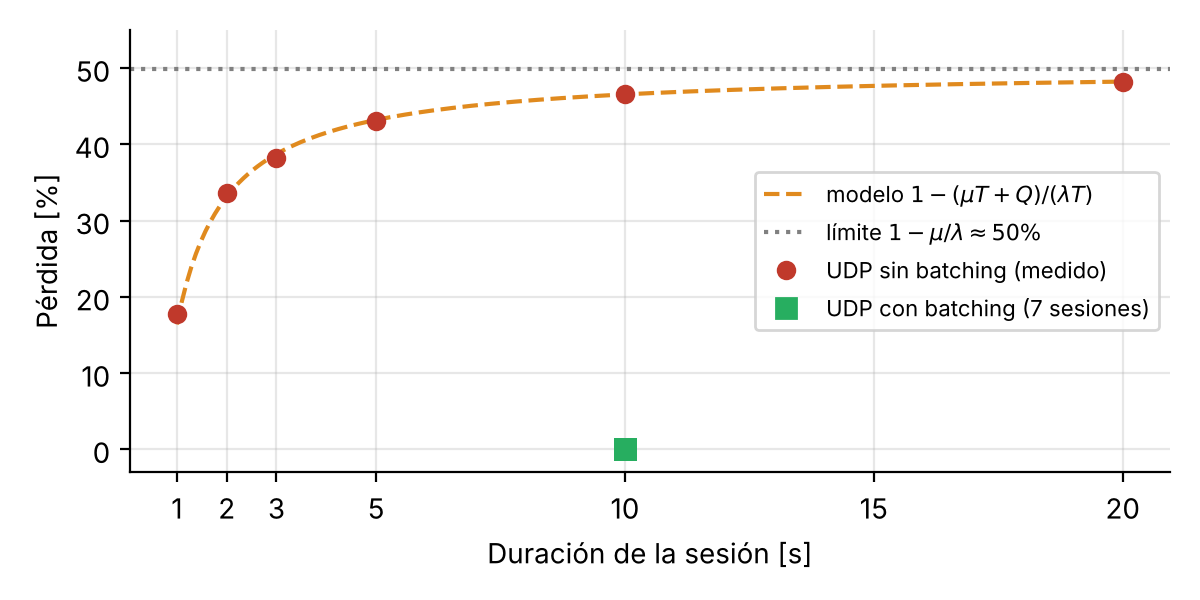
\includegraphics[width=\textwidth]{figuras/perdida_udp.png}\caption{Pérdida UDP a 1600~Hz antes y después del envío por lotes.}
\end{subfigure}\hfill
\begin{subfigure}{0.49\textwidth}\centering
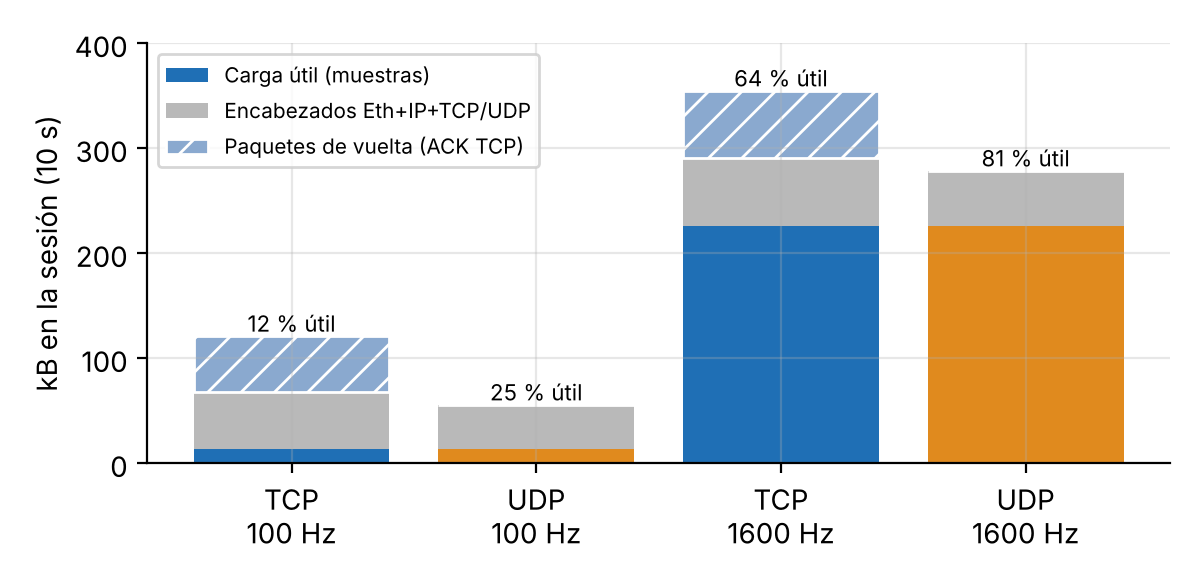
\includegraphics[width=\textwidth]{figuras/bytes_wireshark.png}\caption{Bytes por sesión en las capturas.}
\end{subfigure}\\[4pt]
\begin{subfigure}{0.9\textwidth}\centering
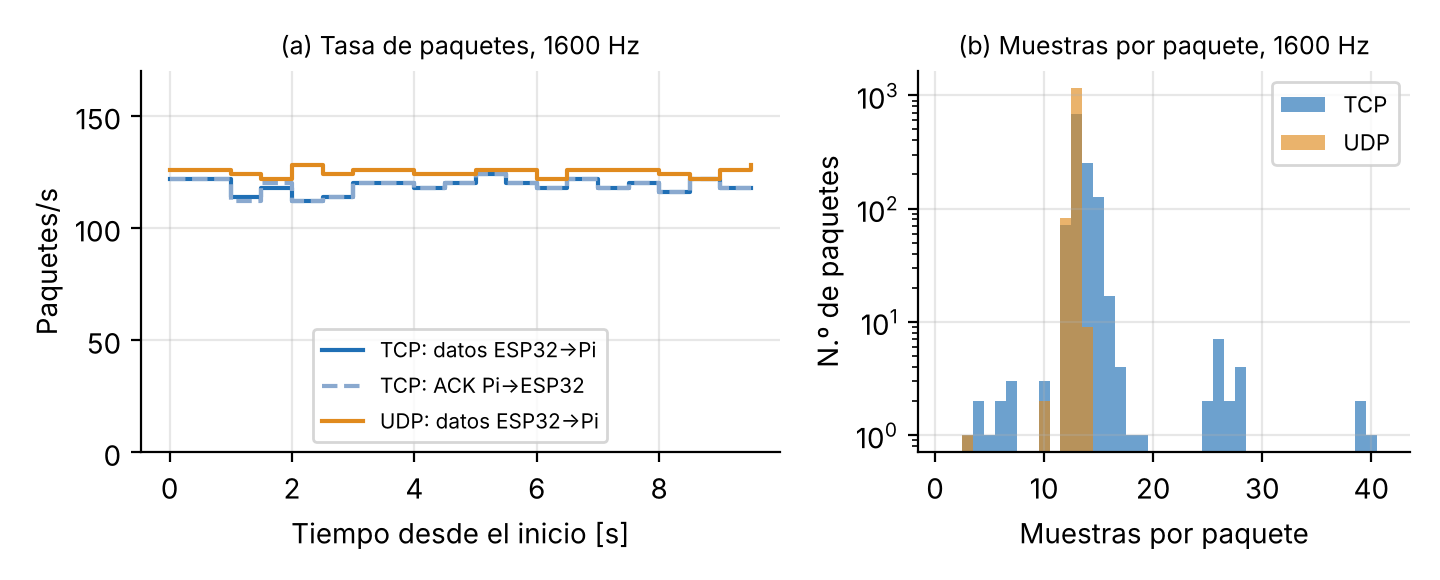
\includegraphics[width=\textwidth]{figuras/wireshark_1600.png}\caption{Capturas a 1600~Hz: paquetes por segundo y muestras por paquete.}
\end{subfigure}
\caption{(a) El modelo de cola (discontinuo) sigue las pérdidas medidas sin parámetros ajustados. (b) Eficiencia de cada protocolo. (c) TCP envía un ACK por segmento y agrupa a su criterio (Nagle); UDP envía una lectura de la FIFO por datagrama.}
\label{fig:resultados}
\end{figure}

\textbf{Análisis.} UDP solo transmite datos; TCP agrega el saludo de tres vías, el cierre con FIN y, aquí, un ACK por segmento. Por eso transmite más bytes para la misma información, sobre todo a 100~Hz (una muestra por paquete: 12\,\% útil frente a 25\,\%). A 1600~Hz, con unas 13 muestras por paquete, la eficiencia $\eta=14n/(14n+H)$ sube al 64 y al 81\,\%. Con enlace corto y baja carga ($\approx$0,2~Mbit/s), ambos entregaron el 100\,\% de las muestras; con pérdidas en el enlace, TCP retransmitiría (más retardo y bloqueo del flujo) y UDP perdería muestras, que \texttt{seq} contabilizaría.

\section{Efecto del rango y de la frecuencia}
\textbf{Rango.} El crudo de 16 bits cubre el rango elegido (ec.~\ref{eq:escala}): la misma gravedad da la mitad de cuentas cada vez que el rango se duplica, mientras que en m/s$^2$ se mantiene (Tabla~\ref{tab:rangofrec}). Un rango pequeño da mejor resolución pero se satura antes: una sesión a $\pm$2~g con movimiento brusco alcanzó 32\,767 (0,03\,\% de muestras recortadas).

\textbf{Frecuencia.} Permite ver vibraciones hasta $f/2$ (Nyquist): 800~Hz a 1600~Hz. A cambio, aumentan los datos ($14f$ B/s: 22,6~kB/s a 1600~Hz) y el ruido, que crece como $\sqrt{f}$ porque el filtro del sensor deja pasar una banda proporcional a $f$. En reposo, a $\pm$16~g, $\sigma$ pasó de 4,5 a $\approx$9 cuentas entre 400 y 1600~Hz: un factor $2=\sqrt{1600/400}$. Para movimientos lentos conviene un rango y una frecuencia bajos; para impactos o vibraciones, altos.

\begin{table}[h]
\centering\small
\caption{Efecto del rango (eje Z, 1~g) y de la frecuencia (ruido en reposo), medidos en \texttt{sensores/}.}\label{tab:rangofrec}
\begin{tabular}{@{}c c c c@{\hspace{1.5em}}c c c@{}}
\toprule
Rango & Cuentas/g teór. & Medidas & 1 cuenta & Configuración & $f$ medida & $\sigma$ \\ \midrule
$\pm$2 g & 16\,384 & 16\,255 & 0,60 mm/s$^2$ & $\pm$2 g, 12,5 Hz & 13 Hz & 0,014 m/s$^2$ \\
$\pm$4 g & 8\,192 & 7\,885 & 1,20 mm/s$^2$ & $\pm$16 g, 400 Hz & 404 Hz & 0,022 m/s$^2$ \\
$\pm$8 g & 4\,096 & 3\,917 & 2,39 mm/s$^2$ & $\pm$16 g, 1600 Hz & 1617 Hz & 0,043 m/s$^2$ \\
$\pm$16 g & 2\,048 & 1\,982 & 4,79 mm/s$^2$ & & & \\ \bottomrule
\end{tabular}
\end{table}

%=====================================================================
\chapter{Limitaciones y conclusiones}
%=====================================================================
\textbf{Limitaciones.} \texttt{t\_us} es estimado; el frame \textit{sensortime} del BMI270, hoy desactivado, permitiría fecharlo mejor. El valor rotulado \textit{jitter} en la GUI es la desviación de \texttt{dt}, no el \textit{jitter} de red. La tasa de la lectura sin FIFO a 400~kHz ($\approx$500/s) es estimada. No se confirmó el origen de los datagramas UDP duplicados (13--26 por sesión, detectados y descartados), y las mediciones de ruido se basan en pocas sesiones en reposo.

\textbf{Conclusiones.} El sistema cumple RF1--RF9. Las decisiones de mayor impacto siguen un mismo principio: pagar el costo fijo de cada operación (una transacción I$^2$C o un paquete) una vez por grupo de muestras y no por cada muestra. La FIFO y el bus a 400~kHz elevaron la adquisición de $\approx$350 a 1617 muestras/s; el envío por lotes eliminó la pérdida de casi el 50\,\% en UDP; y el protocolo binario con \texttt{seq} y \texttt{total} permite contabilizar cualquier pérdida. Wireshark confirma las diferencias teóricas entre TCP (conexión, ACK por segmento, agrupamiento propio) y UDP (solo datagramas).

%=====================================================================
\appendix
\clearpage
\chapter{Anexos}
%=====================================================================
\section{Interfaz web}
\begin{figure}[h]
\centering
\placeholder{0.85\textwidth}{6cm}{Captura de la GUI web durante una sesión a 1600 Hz:\\formulario de configuración, gráfico en vivo, progreso y resumen.}
\caption{Interfaz web de configuración y visualización (RF8).}
\label{fig:gui}
\end{figure}

\break
\section{Capturas de Wireshark}
\begin{figure}[h]
\centering
\begin{subfigure}{0.49\textwidth}\centering
\placeholder{0.95\textwidth}{4.5cm}{Sesión TCP 1600 Hz, filtro\\\texttt{tcp.port==10000}: segmentos\\de datos alternados con ACK.}
\caption{TCP: datos y ACK.}
\end{subfigure}\hfill
\begin{subfigure}{0.49\textwidth}\centering
\placeholder{0.95\textwidth}{4.5cm}{Sesión UDP 1600 Hz, filtro\\\texttt{udp.port==10000}: detalle de un\\datagrama de 182 B en hexadecimal.}
\caption{UDP: datagramas sin respuesta.}
\end{subfigure}\\[6pt]
\begin{subfigure}{0.49\textwidth}\centering
\placeholder{0.95\textwidth}{4.5cm}{Canal de control, filtro\\\texttt{tcp.port==10001}: CONFIG (9 B),\\ACK (1 B) y END (6 B).}
\caption{Mensajes de control.}
\end{subfigure}\hfill
\begin{subfigure}{0.49\textwidth}\centering
\placeholder{0.95\textwidth}{4.5cm}{Statistics $\rightarrow$ Conversations\\o I/O Graph comparando\\TCP y UDP.}
\caption{Estadísticas.}
\end{subfigure}
\caption{Capturas de Wireshark tomadas en la Raspberry Pi.}
\label{fig:wscap}
\end{figure}

\section{Sesiones de prueba en \texttt{sensores/}}
La carpeta contiene unas 60 sesiones con rangos de $\pm$2 a $\pm$16~g, frecuencias de 12,5 a 1600~Hz, ambos transportes y modos, y de 127 a 32\,347 muestras. Algunas representativas:

\begin{center}\small
\begin{tabular}{@{}l c c c c r r@{}}
\toprule
Sesión & Rango & Frecuencia & Transporte & Modo & Muestras & Pérdida \\ \midrule
\texttt{20261008\_203753} & $\pm$2 g & 12,5 Hz & TCP & sec. & 127 & 0\,\% \\
\texttt{20261008\_222936} & $\pm$2 g & 100 Hz & TCP & par. & 506 & 0\,\% \\
\texttt{20261008\_223001} & $\pm$16 g & 400 Hz & TCP & par. & 2\,022 & 0\,\% \\
\texttt{20261008\_222911} & $\pm$16 g & 800 Hz & TCP & par. & 4\,044 & 0\,\% \\
\texttt{20261008\_222809} & $\pm$4 g & 1600 Hz & TCP & sec. & 16\,175 & 0\,\% \\
\texttt{20261010\_102615} & $\pm$2 g & 1600 Hz & UDP & par. & 16\,174 & 0\,\% \\ \bottomrule
\end{tabular}
\end{center}

\section{Uso de herramientas de IA}
Los prompts utilizados, con su etapa, la herramienta y una nota sobre cómo se usó el resultado, se documentan en \texttt{prompts.md}, en la raíz del repositorio.

\end{document}
